
\subsection{Ejercicio 10}

Dadas las implementaciones de $ShedLottery$, con o sin tickets compensatorios (respectivamente en $sched_lottery.cpp$ y $sched_lottery_base.cpp$), el ejercicio nos propone ponerlas a prueba y compararlas, relacion\'andolas con la problem\'atica que presentaban los autores y verificar si los tickets compensatorios son una soluci\'on viable. A continuaci\'on mostramos los experimentos realizados:

\vspace{2mm}

Para comenzar, realizamos experimentaciones sobre lotes ya utilizados en otros ejercicios. Para estos experimentos utilizamos semillas aleatorias ya que es indistinto, y Quantum = 2, de esa forma hay muchos cambios de tarea donde se realizan loter\'ias.

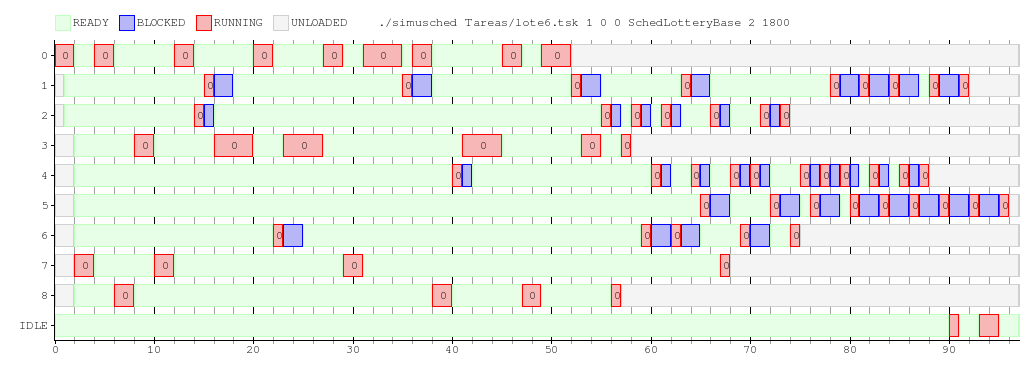
\includegraphics[width=1\textwidth]{./Graficos/Ej10/testBase.png}
\begin{center}
 \textit{Lote = 6, Scheduler = Base, Quantum = 2, Semilla = 1800}.
\end{center}


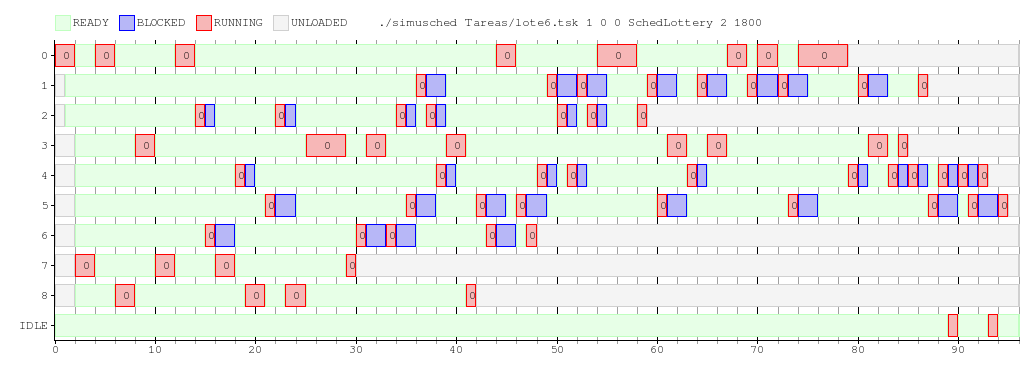
\includegraphics[width=1\textwidth]{./Graficos/Ej10/testComp.png}
\begin{center}
 \textit{Lote = 6, Scheduler = Compensatorio, Quantum = 2, Semilla = 1800}.
\end{center}


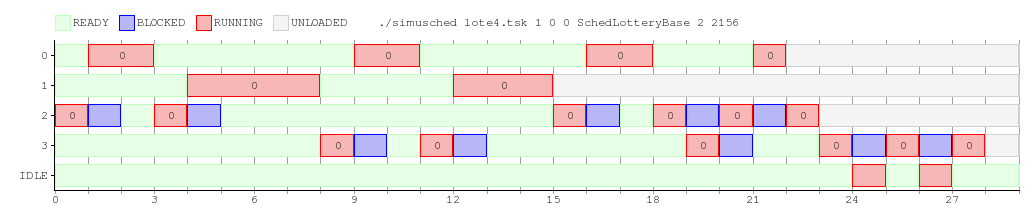
\includegraphics[width=1\textwidth]{./Graficos/Ej10/testBase2.png}
\begin{center}
 \textit{Lote = 4, Scheduler = Base, Quantum = 2, Semilla = 2156}.
\end{center}


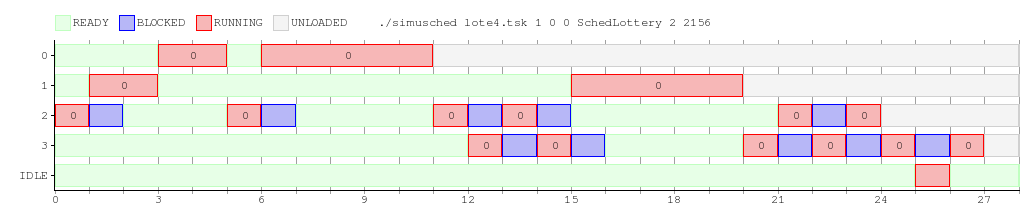
\includegraphics[width=1\textwidth]{./Graficos/Ej10/testComp2.png}
\begin{center}
 \textit{Lote = 4, Scheduler = Compensatorio, Quantum = 2, Semilla = 2156}.
\end{center}

	

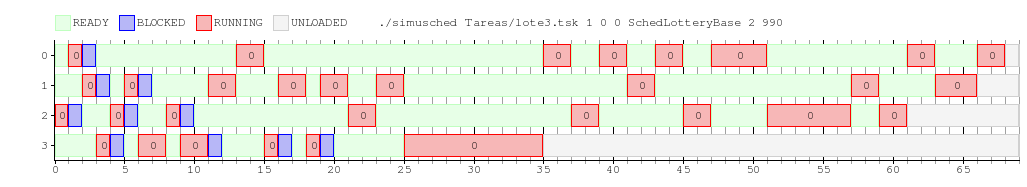
\includegraphics[width=1\textwidth]{./Graficos/Ej10/testBase3.png}
\begin{center}
 \textit{Lote = 3, Scheduler = Base, Quantum = 2, Semilla = 990}.
\end{center}


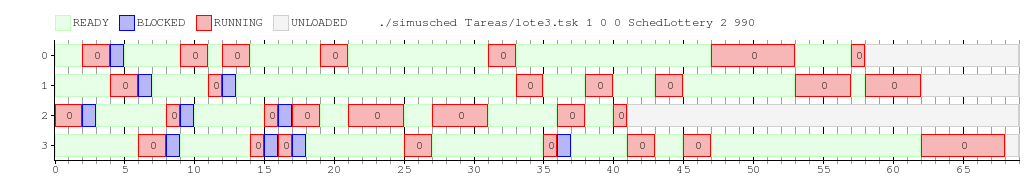
\includegraphics[width=1\textwidth]{./Graficos/Ej10/testComp3.png}
\begin{center}
 \textit{Lote = 3, Scheduler = Compensatorio, Quantum = 2, Semilla = 990}.
\end{center}

\vspace{2mm}

Para este test generamos un lote de tareas nuevo, en el cual ejecutamos 3 tareas de uso intensivo de CPU por 30 ticks, y 2 tareas TaskConsola que realicen 10 llamadas bloqueantes de 1 tick de duraci\'on, 


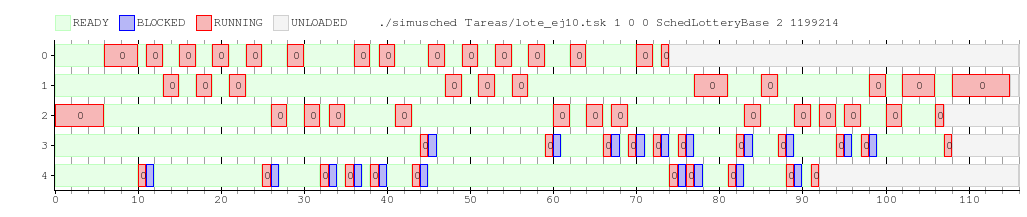
\includegraphics[width=1\textwidth]{./Graficos/Ej10/testBase5.png}
\begin{center}
 \textit{Lote = ej10, Scheduler = Base, Quantum = 2, Semilla = 1199214}.
\end{center}


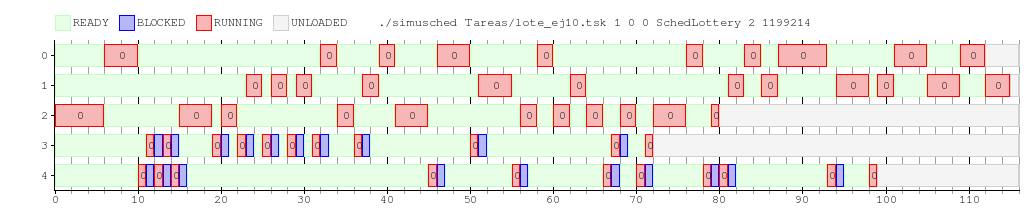
\includegraphics[width=1\textwidth]{./Graficos/Ej10/testComp5.png}
\begin{center}
 \textit{Lote = ej10, Scheduler = Compensatorio, Quantum = 2, Semilla = 1199214}.
\end{center}


Puede apreciarse en todos los casos como en el scheduler base, las tareas que utilizan IO se amontonan en el final de la ejecuci\'on, bloque\'andose y no retomando control del cpu hasta mucho despu\'es. En cambio, en el scheduler compensatorio pueden apreciarse algunas tareas en la mitad de la ejecuci\'on que luego de desbloquearse vuelven a tomar control de la CPU, gracias a la compensaci\'on.
